\documentclass[10pt,a4paper]{article}
%standard symbols
\usepackage{amssymb, amsmath, esint, mathrsfs, tipa}
%charts and tables
\usepackage{array, enumitem}
%graphics
\usepackage{graphicx}
%packages for float
\usepackage{wrapfig, placeins, float}
%specialized tools
\usepackage[americanvoltages,RPvoltages]{circuitikz}
%geometry
\usepackage[left=2.0cm, right=2.0cm, top=2.5cm]{geometry}
%code
\usepackage{listings}
%links
\usepackage{hyperref}

\setlength{\textfloatsep}{5pt plus 2pt minus 2pt}
\setlength{\floatsep}{5pt plus 2pt minus 2pt}

\begin{document}

%\tableofcontents

\section{Introduction and CSC Overview}

These are a collection of personal notes on the optical data acquisition motherboard (ODMB), a circuit board used by the CMS CSC detectors, and related background. A good introduction to the CSCs and ODMB topics is given by \href{https://indico.cern.ch/event/750612/}{Manuel's ODMB Lecture Series}.

\subsection{CMS Muon System}

%Intro to muons
Muons are arguably the most important physics probe at the LHC. Muons offer the cleanest experimental signature of any fundamental particle since they are directly detected and they suffer from less radiative losses than electrons due to their larger mass. Moreover, prompt muons are only generated through off-shell photons and W, Z, and Higgs bosons. This makes them an excellent probe for studying various physics processes due to their ability to suppress large QCD multijet backgrounds.

%Intro to CMS muon system
The main goals of the CMS muon detectors are to identify muons, provide a momentum measurement, and to provide triggering capabilities. CMS detects muons using a system of muon chambers that are located on the outside of the experiment, past the calorimeters and solenoid magnet. Most electrically charged particles and hadrons produced in proton-proton collisions are stopped by the calorimeters, leaving only muons to be detected by the muon chambers. The muon chambers are interwoven with the CMS solenoid magnet's return yoke allowing for momentum measurement by measuring the curvature of the muons' trajectories in the magnetic field. The muon chambers also interface with the level-1 trigger system, which constructs tracks using information from the muon chambers and uses this information along with information from the calorimeters to decide whether or not data should be read out and sent to the data acquisition system.

%Intro to muon detector types
CMS uses four different technologies for detecting muons, which form subgroups within the greater muon detector group. All of the muon detectors are gaseous ionization chambers. Muons ionize the gas in the detectors and the freed electrons drift to an area of high electric field where they initiate an avalanche that amplifies the signal to detectable levels. As an example, the cathode strip chambers currently use a gas mixture of 40\% Ar to produce ionization, 50\% CO$_2$ as a quenching gas to suppress spurious pulses from photons, and 10\% CF$_4$ to prevent polymerization on the surface of the strips. CF$_4$ is a hazardous greenhouse gas, and there are currently studies on reducing its usage. The primary background in the muon chambers is from neutrons, which can collide with nuclei and produce photons, which then pair produce or ionize atoms.

In the barrel region ($|\eta|<1.2$) muons are detected by drift tubes (DTs), which are comparatively cheap and capable of making relatively precise measurements. DTs consist of long cells with an anode wire suspended in the middle of the cell. Muons passing through a DT will ionize the gas, and the freed electrons will drift toward the anode, initiating an avalanche when they approach the anode. By measuring the drift time of the electrons, an accurate measurement of muon position can be obtained. 

In the endcap region ($0.9\leq |\eta|<2.4$) cathode strip chambers (CSCs) are employed due to the higher muon and background rates. CSCs are also able to make relatively precise measurements of muon tracks and can operate in the higher flux region closer to the beam line, though they are also more expensive than DTs. CSCs consists of 6 layers of anode wires between 7 layers of cathode strips, which are angled relative to the anodes. When a muon passes through a CSC, it ionizes the gas and the resulting electrons drift toward the anode wires, initiating an avalanche when they reach one. The subsequent avalanche generates positive ions, which induce a charge on the adjacent cathode. The muon position can then be determined by which anode wires and cathode strips measure a current. Note that multiple muons passing through the same CSC will introduce ambiguity of which anode signals and cathode signals correspond, also known as `ghosts'.

The CSCs and DTs are supplemented over the range $|\eta|<1.6$ (to be upgraded to $|\eta|<2.4$ before phase II) by resistive plate chambers (RPCs), which provide coarser position measurements but can provide more precise timing measurements for triggering. An RPC gap contains a gas mixture surrounded by two resistive plates coated with conductive outer layers to which a large voltage is applied. Muons passing through the gap ionize the gas an initiate an avalanche, which induces a current on these outer layers. 

Finally, the phase II upgrades introduced the gas electron multipliers (GEMs) in the very forward region ($1.6\leq |\eta|<2.4$ with eventual extension to $1.6\leq |\eta|<2.8$). GEMs provide precise measurements and can withstand the high flux in this region. GEMs have three thin polymer foils coated with copper on either side and perforated with micro-holes. When a muon passes through the chamber and ionizes the gas, the electrons drift toward the holes, which have a strong electric field due to the large voltage applied across the conductive layers on the foil. This causes an avalanche, amplifying the number of electrons. This is repeated 3 times and eventually, the electrons are detected by an electrode on the side of the chamber.

%Detector numbering
Figure~\ref{fig:muonchambers} shows a R-Z cross section of the CMS detector as it will during phase II. DT stations, shown in orange, are denoted as MB\#$\pm$ \# where MB stands for ``muon barrel'', the first number is the station with 1 being the innermost station and 4 the outermost station, and the second number is the wheel (-2 to 2). Each DT station is associated with an RPC station, shown in blue, which uses the same naming scheme except with RB for ``RPC barrel'' rather than MB. CSC stations, shown in green, are denoted as ME$\pm$\#/\# where ME stands for ``muon endcap'', the first number denotes the endcap disk with 1 being the closest disk and 4 being the furthest disk and the sign denoting which endcap side, and the second number denotes the radial station. Some CSC stations are adjacent to RPC stations, shown in blue and violet, which employ a similar naming scheme, but with RE for ``RPC endcap''. The ME$\pm$1/1 and ME$\pm$2/1 CSC stations are adjacent to GE$\pm$1/1 and GE$\pm$2/1 GEM stations, shown in red. In the very foward, there is the ME$\pm$0 GEM station, shown in orange.

\begin{figure}[H]
\centering
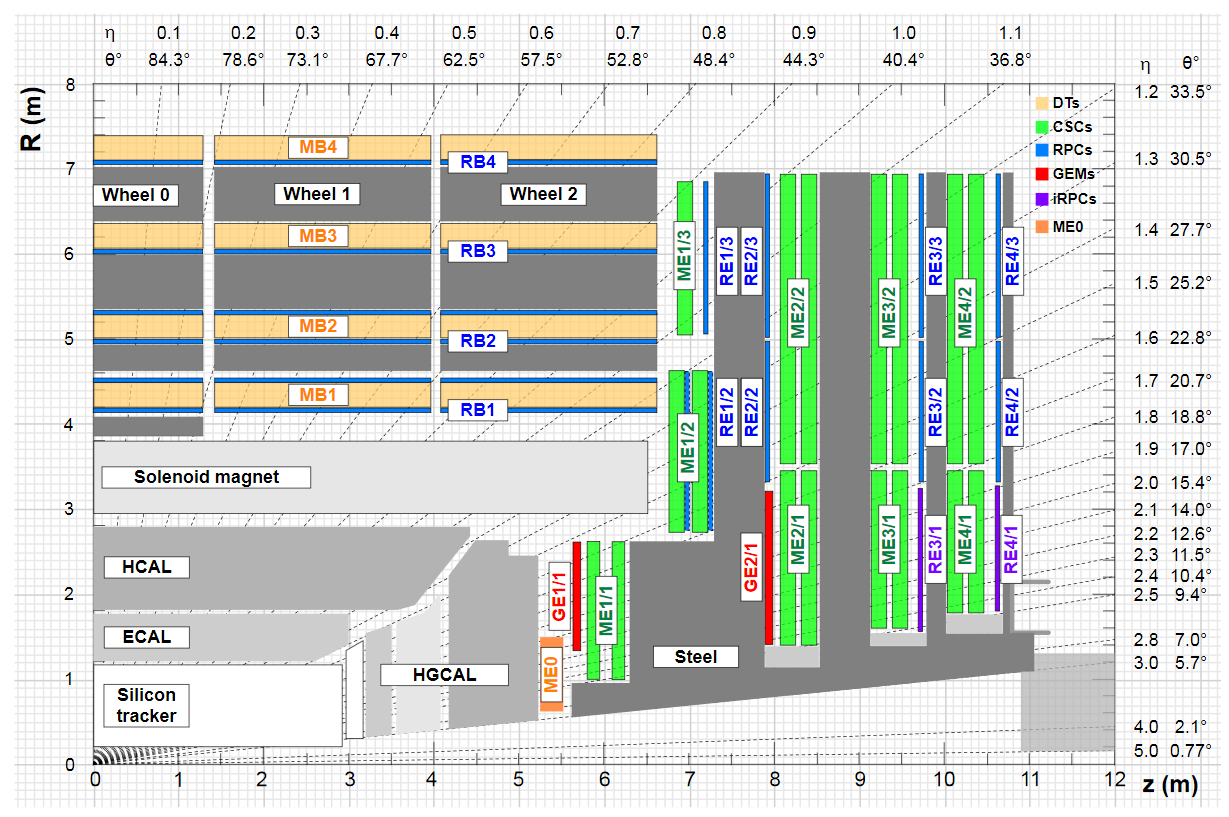
\includegraphics[width= 0.8 \textwidth]{figures/muonchambers.png}
\caption{R-Z cross section of the CMS detector as it will appear in phase II}
\label{fig:muonchambers}
\end{figure}

\subsection{CSC Chambers}

%CSC versions, hardware, and upgrades
The CSC detectors and electronics at the different stations differ due to both detector geometry and physics considerations. The ME$\pm$1/1, ME$\pm$1/2, ME$\pm$1/3, ME$\pm$2/2, ME$\pm$3/2, and ME$\pm$4/2 stations each have 36 chambers per station while the ME$\pm$2/1, ME$\pm$3/1, and ME$\pm$4/1 (collectively called ME$\pm$x/1) stations each have 18 chambers per ring. An individual CSC chamber is denoted as ME$\pm$\#/\#/\# with the third number denoting the specific chamber in the station. The ME$\pm$1/1 chambers are particularly special since they are the innermost detectors which means they see the highest particle flux per area as well as experience the magnetic field of the main solenoid. The ME$\pm$1/1s have different gas and wire spacings, and due to the solenoid's magnetic field, they are the only chambers whose anode wires and cathode strips are not at right angles. It was found after run 1 that the ME$\pm$1/1 electronics were barely able to cope with the LHC particle rate and new electronics were installed during LS 1 to mitigate the problem. The ME$\pm$4/2s were also installed for the first time during LS 1. In order to cope with the much higher particle rates during phase II, the CSC electronics are again being upgraded. In particular, the phase II level-1 trigger may operate at a rate of around 500 kHz, compared to 100 kHz for phase I and have a latency of 12.5 $\mu$s compared to 3.2 $\mu$s for phase I. 

%Power
The high voltages applied across the anodes wire and cathode strips are supplied by the high voltage system. The voltage from the primary supply is supplied to several master distribution cards in USC, each of which supplies voltage to several remote distribution cards in UXC, which then supply the voltage to the chambers. The ME$\pm$1/1s operate at a voltage of 2.9 kV while the other chambers operate at 3.6 kV due to their larger gaps. These values were picked to maximize the charge produced in an avalanche while minimizing the aging of the chambers. The low voltage system begins with the CMS uninterruptible power supply (UPS), which supplies AC power to the power factor converter (OPFC) in UXC. The OPFC converts this to 385 DC and sends it to Maraton (magnetic and radiation tolerant) power supplies in UXC, which supply power both to the CSC peripheral crates as well as to the junction boxes connected to the on-chamber electronics. 

\subsection{CSC Electronics}

%CSC electronics
The CSC electronics boards are split between those mounted on the chambers and those located in VME peripheral crates attached to the outside of the CMS detector as shown in figure~\ref{fig:cscelectronics}. The anode front-end boards (AFEBs), cathode front-end baords (CFEBs), anode local charged track boards (ALCTs), and low voltage distribution boards (LVDBs) are located on the chamber while the timing motherboards (TMBs), data acquisition motherboards (DMBs), VME crate controllers (VCCs), muon port cards (MPCs), and clock control boards (CCBs) are located in the VME crates. 

\begin{figure}[H]
\centering
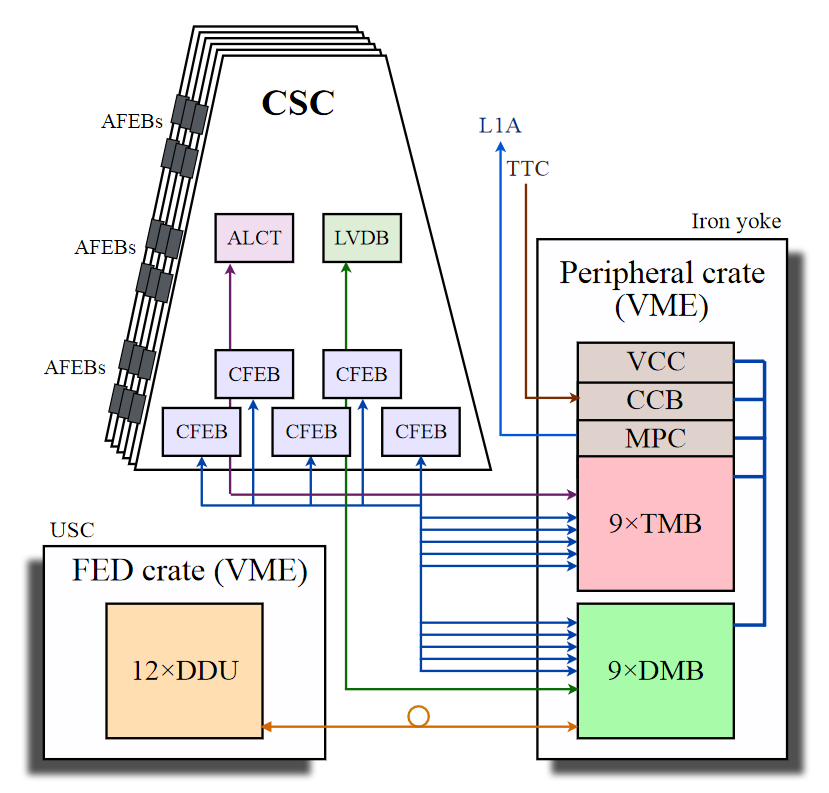
\includegraphics[width= 0.6 \textwidth]{figures/cscelectronics.png}
\caption{Original electronics boards associated with CSCs}
\label{fig:cscelectronics}
\end{figure}

%AFEBs and ALCTs
The anode wires of CSCs are bunched into wire groups (WGs) of 10-15s wires, which are connected to AFEBs. There are 12-42 AFEBs per chamber, depending on chamber type, and each AFEB possesses a 16-channel amplifier-discriminator ASIC that converts the signals on the anode wires to 40 ns single bit digital pulses. These pulses are sampled every 25 ns by the ALCT, which stores the AFEB outputs in a FIFO and also scans the anode outputs for preset patterns that would be consistent with muon tracks. Such patterns are called anode local charged tracks (confusingly also abbreviated ALCTs), which are then passed to the TMB in the peripheral crate. The ALCT boards consist of two parts, a baseboard that receives the AFEB signals and aligns them with 2.2 ns precision, and the mezzanine, which has the FPGA and handles the FIFOs and searching for ALCTs. The ALCT-288 baseboard is used for the ME$\pm$1/123s, the ALCT-384 baseboard for the ME$\pm$x/2s, and the larger ALCT-672 baseboard for the ME$\pm$x/1s. Originally, the ME$\pm$x/1s had ALCT-E1000 mezzanines while the others were equipped with ALCT-600E mezzanines. During the LS1 upgrades, the ME$\pm$1/1s received new ALCT-LX150 (also known as ALCT-S6) mezzanines, as did the ME$\pm$4/2s that were being installed for the first time. The phase II upgrades require most ALCT mezzanines to be upgraded to account for increased trigger latency and improve bandwidth. The ME$\pm$1/1s received new ALCT-LX100 mezzanines with optical readouts using GBTx transceivers; ME$\pm$1/2 and ME$\pm$23/2 also have ALCT-LX100 mezzanines but will use copper readout. The ME$\pm$x/1s received ALCT-LX150T mezzanines with optical readout using GBTx transceivers. Finally, the old ME$\pm$1/1 ALCT-LX150 mezzanines were moved to the ME$\pm$1/3s. 

%CFEBs
There were originally 4-5 CFEBs per chamber. The CFEBs first have a Buckeye amplifier-shaper that sends the resulting amplified signals to two different paths. On the trigger path, a comparator network checks signals from triples of adjacent strips and is able to locate muon hits to a resolution of half a strip. These comparator half-strip hits are then sent to the TMB. On the DAQ path, an SCA chip samples the amplifier-shaper output every 50 ns and stores the result on its capacitors, storing up to 6 events worth of data. Upon receiving an accept signal, the 8 to 16 samples in the appropriate time window are digitized by a ADC and sent to the DMB. During LS1, ME$\pm$1/1s were upgraded to have 7 digital cathode front-end boards (DCFEBs). DCFEBs immediately digitize the output of the amplifier-shapers which are then sent to comparator ASICs and a Virtex-6 FPGA with a large buffer. DCFEBs are equipped with Finisar transceivers to send optical data to OTMBs and ODMBs. For phase II, the ME$\pm$x/1 chambers will receive DCFEBs while the ME$\pm$1/1 chambers will receive the more radiation hard xDCFEBs, which are equipped with VTTx and VTRx transceivers, the latter of which enables PROM-less programming should the xDCFEB PROM die from radiation. There are also plans to replace the finisars on the DCFEBs with VTTx and VTRx for improved radiation resistance. 

%TMBs and MPCs
For each chamber, there is one TMB, located in the peripheral crate. The TMB receives data from ALCTs (via an intermediate RAT board) and CFEBs. Using the comparator half-strip hits from the CFEBs, the TMB searches for patterns to construct cathode local charged tracks (CLCTs), similarly to the ALCTs, and then matches CLCTs and ALCTs to form 2D-LCTs. The 2D-LCTs from groups of 9 chambers in a sector are sent to the MPC, which selects the 3 highest quality candidates to send to the endcap muon track finder (EMTF) in the trigger system. Like the ALCTs, the TMBs have a separate baseboard and mezzanine. During LS1, the ME$\pm$1/1 TMBs were replaced with optical timing mother boards (OTMBs) controlled by Virtex-6 FPGAs and equipped with Snap12 receivers for receiving optical data from the DCFEBs. For the phase II upgrades, the TMBs for the ME$\pm$x/1s will be replaced with OTMBv2s capable of receiving optical data from the on-chamber electronics. 

%DMBs, DDUs, and DAQ
There is also one DMB associated to each chamber, again located in a peripheral crate. The DMBs are controlled with two Spartan-2 FPGAs. Upon receiving a level-1 accept (L1A) from the trigger system, the DMB checks if there are any ALCTs or CLCTs within a programmable window of the L1A. If there is an L1A-LCT coincidence, data is read out from the ALCTs, CFEBs, and TMBs. The DMB sends an event record including hits, LCT decisions, and board status via a Finisar transceiver to a detector dependent unit (DDU) in a FED crate in USC. Each DDU combines the data from 15 DMBs and performs error checking before sending the data to a data concentration card (DCC), which finally sends the data to a CMS filter farm. During LS1, the ME$\pm$1/1 chambers had their DMBs replaced by optical data acquisition motherboards (ODMBs). ODMBs are controlled by a Virtex-6 FPGA and can receive data from the 7 DCFEBs via Snap12 optical receivers. Slow control signals to the 7 DCFEBs are multiplexed by patch-patch interconnecting boards (PPIBs). The 1.6 Gb/s optical link to the DDUs was retained from the DMBs, but this will be insufficient during phase II. The phase II upgrades include replacing the current ODMBs with ODMB7s featuring firefly optical receivers receiveing data from the xDCFEBs and ALCTs and receivers sending data to the DDUs as well as replacing the ME$\pm$x/1 DMBs with similar ODMB5s. The back-end including the DDUs will also be replaced for the phase II upgrades.

%LVDB
The LVDB is an on-chamber circuit board which supplies low noise voltages to the various on-chamber electronics. Like the ALCT and TMB, the LVDB has a separate baseboard and mezzanine, the low voltage mezzanine board (LVMB). During LS1, the LVDBs and LVMBs in ME$\pm$1/1s were upgraded to LVDB7s and LVMB7s to handle the 7 DCFEBs. During LS2, the LVDBs in the ME$\pm$x/1s were upgraded to LVDB5s to handle DCFEBs.

%VCC, CCB
The peripheral crates also contain VCCs and CCBs. VCCs receive commands from detector operators and communicate them to the other boards in the crate, which then communicate with the on-chamber electronics. CCBs distribute central CMS signals like the central clock and L1As, which they receive from the central TCDS (timing and control distribution system). 

\section{ODMB Functionality and Relevant Protocols}

\subsection{Data Format}

%DDU data format
The main purpose of the ODMB during CMS data taking is packet building. The ODMB receives signals from the OTMB when LCTs are constructed. When the ODMB receives an L1A from the CCB, it checks if there is a matching LCT. If this is the case, the ODMB considers it an L1A\_MATCH and immediately issues a header to the DDU and begins reading data from the DCFEBs, ALCT, and OTMB. The ODMB then transfers the ALCT data, the OTMB data, and the relevant DCFEB data in that order followed by the tailer.

\subsection{VME Protocol}

Slow control commands are issued to the ODMB and other VME boards from the VCC via the VME backplane using the VME64 protocol. A VME peripheral crate will have a 1 VCC, 1 CCB, 1 MPC, 9 DMBs, and 9 TMBs as specified in table~\ref{tab:vmecrate}. The ODMB and OTMB associated to each chamber are in adjacent slots in the VME crate; there are custom buses on the backplane that allow ODMBs to communicate with the adjacent OTMB as well as the CCB. The signals transmitted through the standard VME backplane are detailed in table~\ref{tab:vmeinterface} with those used by the ODMB listed above the double horizontal line. 

\begin{table}[H]
\centering
\begin{tabular}{|l|l|l|} \hline
Slot Number& Board& Paired Board\\ \hline
1& VCC & \\ \hline
2& (O)DMB & (O)TMB in slot 3 \\ \hline
3& (O)TMB & (O)DMB in slot 2 \\ \hline
4& (O)DMB & (O)TMB in slot 5 \\ \hline
5& (O)TMB & (O)DMB in slot 4 \\ \hline
6& (O)DMB & (O)TMB in slot 7 \\ \hline
7& (O)TMB & (O)DMB in slot 6 \\ \hline
8& (O)DMB & (O)TMB in slot 9 \\ \hline
9& (O)TMB & (O)DMB in slot 8 \\ \hline
10& (O)DMB & (O)TMB in slot 11 \\ \hline
11& (O)TMB & (O)DMB in slot 10 \\ \hline
12& CCB & \\ \hline
13& MPC & \\ \hline
14& (O)TMB & (O)DMB in slot 15 \\ \hline
15& (O)DMB & (O)TMB in slot 14 \\ \hline
16& (O)TMB & (O)DMB in slot 17 \\ \hline
17& (O)DMB & (O)TMB in slot 16 \\ \hline
18& (O)TMB & (O)DMB in slot 19 \\ \hline
19& (O)DMB & (O)TMB in slot 18 \\ \hline
20& (O)TMB & (O)DMB in slot 21 \\ \hline
21& (O)DMB & (O)TMB in slot 20 \\ \hline
\end{tabular}
\caption{Boards in a CSC peripheral crate}
\label{tab:vmecrate}
\end{table}

\begin{table}[H]
\centering
\begin{tabular}{|l|l|} \hline
VME Signal& Description\\ \hline
\texttt{d}& 16 bit data bus, used to transfer data both to and from the slave.\\ \hline
\texttt{a}& 23 bit address bus, the first five of which are used to choose the slot in the crate\\
                  & being addressed and the latter 18 of which define the command issued.\\ \hline
\texttt{am}& 6 bit address modifier. Specifies command type.\\ 
\texttt{ga}& 5 bit geographical address. Static and unique to each VME slot.\\ \hline
\texttt{gap}& Geographical address parity. 1 if \texttt{vme\_ga} has an even number of \\
                 & 1's and 0 otherwise. \\ \hline
\texttt{as\_b}& Address strobe (bar). Indicates \texttt{vme\_addr} is ready to be read. \\
\texttt{ds\_b}& 2 bit data strobes (bar). Each corresponds to one byte of \texttt{vme\_data} \\
                   & and indicates the data is ready to read. \\
\texttt{sysfail\_b}& Sysfail (bar) signal indicating a failure of the VME system. \\
\texttt{berr\_b}& Error (bar) signal indicating and error in the VME system and postpones \\
                     & any commands.\\ \hline
\texttt{iack\_b}& Interrupt acknowledge (bar). Commands should only be accepted while \texttt{IACK}\\
                     & is high, allowing the master to interrupt commands by driving it low. \\ \hline
\texttt{lword\_b}& Load word (bar). Defines size of data transfers \\ \hline 
\texttt{write\_b}& Write (bar). Indicates if the current command is a read or write command.\\ \hline
\texttt{dtack\_b}& Data acknowledge (bar). Driven by slave when command is received or\\
                          & when data is ready to be read for read commands.\\ \hline
\texttt{gnd}& VME ground. \\ \hline
\texttt{v\#}& Standard voltage pins for powering the board. \\ \hline \hline

\texttt{acfail\_b}& AC fail (bar). Indicates problems with VME power supply.\\ \hline
\texttt{bbsy\_b}& Bus busy (bar). Driven by slave to claim bus and indicate usage.\\ \hline
\texttt{bclr\_b}& Bus clear (bar). Asserted to indicate a board wishes to use a bus that is currently \\
                & in use.\\
\texttt{bg\#in\_b}& 4 bus grant input (bar) signals. The bus grant system is daisy chained i.e.\\
               & \texttt{bg\#in\_b} is connected to \texttt{bg\#out\_b} from the board in the previous\\ 
							 &  VME slot. Driven by the controller to indicate bus usage has been granted.\\ \hline
\texttt{bg\#out\_b}& 4 bus grant output (bar) signals. See \texttt{bg\#in\_b}.\\ \hline
\texttt{br\#\_b}& 4 bus request (bar) signals. Driven low to indicate to controller board is\\
                & requesting use of a bus.\\ \hline
\texttt{iackin\_b}& Interrupt acknowledge input (bar). Daisy chained i.e. connected from \texttt{iackout\_b}\\
               & of the board in the previous slot. Indicates an interrupt acknowledge in progress.\\ \hline
\texttt{iackout\_b}& Interrupt acknowledge output (bar). See \texttt{iackin\_b}.\\ \hline
\texttt{irq\#\_b}& Interrupt request (bar). Used to request interrupt from controller.\\ \hline
\texttt{li/i\_b}& Live insertion input (bar). Can be used for control when hot swapping boards.\\ \hline
\texttt{li/o\_b}& Live insertion output (bar). Can be used for control when hot swapping boards.\\ \hline
\texttt{tm}& 5 bits used to implement the MTM protocol for communication.\\ \hline
\texttt{resp\_b}& Response (bar). Used by the 2eVME protocol to speed up data transfers. \\ \hline
\texttt{rsvbus}& Reserved bussed signal. Should not be used. \\ \hline
\texttt{rsvu}& Reserved unbussed signal. Should not be used. \\ \hline
\texttt{retry\_b}& Retry (bar). Can be used with \texttt{berr\_b} to postpone the current command\\
                 & and request the master retry at a later time.\\ \hline
\texttt{sba}& Serial A. Can be used for any user-defined serial bus protocol.\\ \hline
\texttt{sbb}& Serial B. Can be used for any user-defined serial bus protocol.\\ \hline
\texttt{serclk}& Serial clock. Can be used for any user-defined serial bus protocol.\\ \hline
\texttt{serdata}& Serial data. Can be used for any user-defined serial bus protocol.\\ \hline
\texttt{sysclk}& 16 MHz clock. Not related to other VME signals.\\ \hline
\texttt{sysreset\_b}& System reset (bar). Indicates reset in progress.\\ \hline
\texttt{vpc\#}& Voltage pre-contact pins. Connect first and disconnect last so they can be used\\
              & for pre-charge power sources during hotswaps.\\ \hline
\texttt{v5pstdby}& Standby power supply connected to a rechargeable battery.\\ \hline
\end{tabular}
\caption{Signals in VME interface}
\label{tab:vmeinterface}
\end{table}

The ODMB only uses commands sent with AM code \texttt{111010}, which corresponds to a 24 bit non-privileged instruction, and LWORD asserted i.e. 16 bits of data. This means that both data strobe lines are used. The 23 bits on the address bus are extended to 24 bits by appending a 0 to the end. The first 5 bits of the address then indicate the slot number being addressed with \texttt{11111} indicating a broadcast to all slots. The lower 18 bits plus the implicit last bit correspond to the command issued. Thus, an address signal \texttt{01010000010000010000000} (0x282080) should be interpreted as addressed to slot \texttt{01010} (10) and containing the command \texttt{0000100000100000000} (0x04100). The fourth hex digit of the command, 0x4 in the previous example, indicates the module within the ODMB to which the command is addressed. This is discussed in more detail in the firmware section below.

The VME communication process occurs in several steps, an example of which is shown in figure~\ref{fig:vmewrite}. The steps for a VME communication are detailed below. Note that the ODMB only uses single-cycle commands, so step 6a is never used in the case of commands issued to the ODMB.

\begin{enumerate}
\item The master drives status signals like \texttt{am} and \texttt{lword\_b}. \texttt{iack\_b} is driven high and the address \texttt{a} is loaded. 
\item After \texttt{a} is valid for at least 35 ns, the master can drive \texttt{as\_b} low to indicate address is ready to read
\item Drive \texttt{write\_b} signal. If the command is a write command, drive data \texttt{d} signals as well.
\item After DATA is valid for at least 35 ns and both \texttt{dtack\_b} and \texttt{berr\_b} are high, drive one or both \texttt{ds\_b} lines low to indicate data is ready to read.
\item For a write command, when slave has read data, it drives \texttt{dtack\_b} low. For a read command, once the slave has presented data on \texttt{d} for 35 ns it can drive \texttt{dtack\_b} low.
\item The next step for the master depends on whether it is the last cycle of the command or if there are more.
\begin{itemize}
\item If performing a multi-cycle command and it is not the last cycle, once \texttt{dtack\_b} has been low for 10 ns, the master drives the \texttt{ds\_b} lines high. This is received by the slave, which
 releases \texttt{dtack\_b} and when this is received by the master, the process returns to step 3.
\item For the last cycle, once \texttt{dtack\_b} has been low for 10 ns, master (VCC) can release \texttt{a}, \texttt{am}, \texttt{lword\_b}, \texttt{iack\_b}, and \texttt{d}. \texttt{ds\_b} are driven  high.
\end{itemize}
\item When slave receives \texttt{ds\_b} high, it releases \texttt{dtack\_b}. 
\item When the master receives \texttt{dtack\_b} high, it can drive \texttt{as} high, then release all lines.
\end{enumerate}

\begin{figure}[H]
\centering
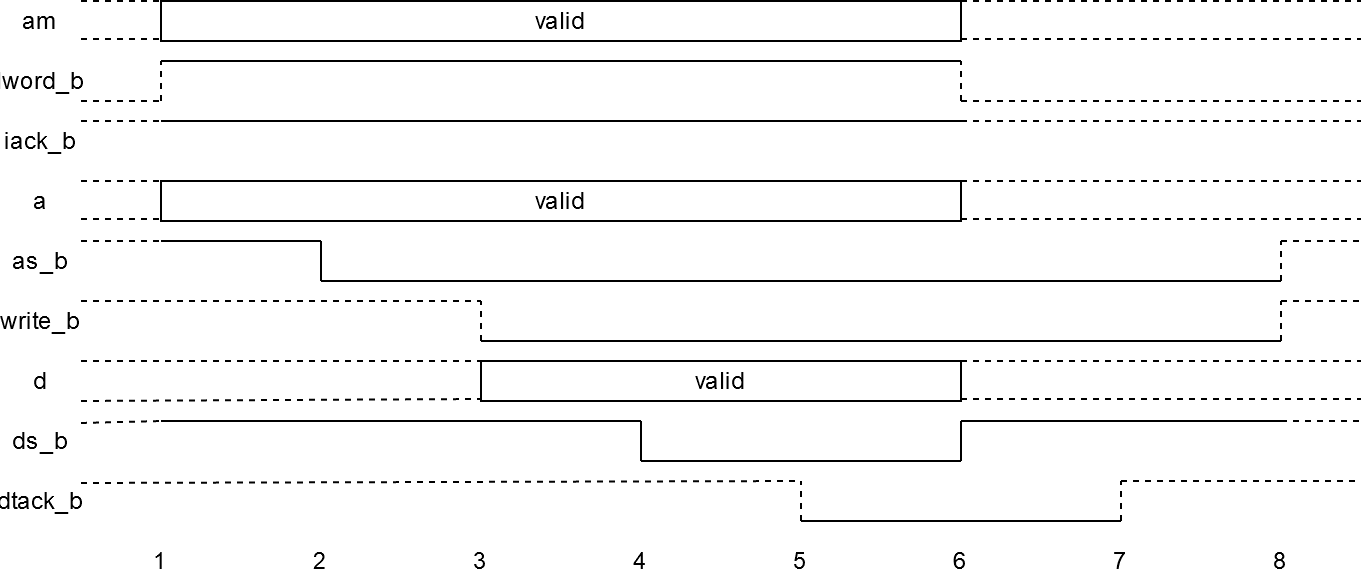
\includegraphics[width= 0.8 \textwidth]{figures/vmeprotocol.png}
\caption{Example of a single cycle 16 bit write. Note the time axis is only schematic and is not to scale.}
\label{fig:vmewrite}
\end{figure}

\subsection{JTAG Protocol}

The JTAG protocol is used in several points throughout the CSC electronics. It is used by the (O)DMBs to communicate with the (x)(D)CFEBs, it is used by computers to program boards using the Xilinx red box, and it can be used by the VCC when boards are not responding via the usual VME protocol. The protocol uses only 4 signals, called TMS, TCK, TDI, and TDO. Typically, a controller will distribute TCK and TMS signals to all modules being controlled while the TDI and TDO are connected in a daisy chain, shown in figure~\ref{fig:jtagdaisychain} for the example of the ODMB and xDCFEB, which has 5 internal modules daisy chained together.

\begin{figure}[H]
\centering
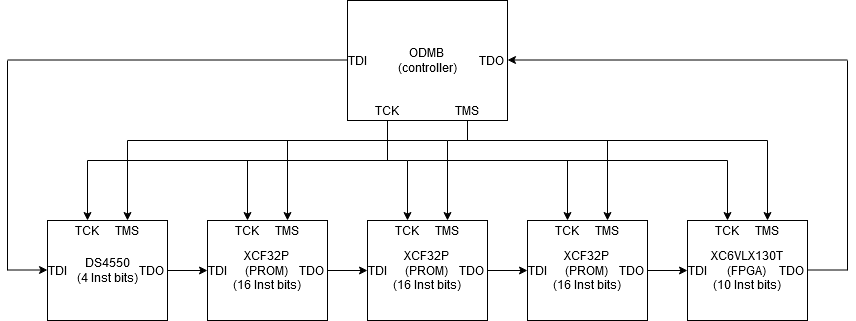
\includegraphics[width= 0.75 \textwidth]{figures/jtagdaisychain.png}
\caption{Diagram of JTAG daisy chain for xDCFEBs. Unlike DCFEBs, which have a single device, the FPGA, in the chain, xDCFEBs have 5 devices, each with a specified length instruction register.}
\label{fig:jtagdaisychain}
\end{figure}

The controller operates the TCK clock and the modules being controlled respond based on the value of TMS at each rising edge of TCK according to a state machine shown in figure~\ref{fig:jtagstatemachine}. The two main actions one typically enacts with JTAG are transferring to and from the data register (DR) and transferring to and from the instruction register (IR). Each time the state machine is in the ``shift DR'' state and a rising TCK edge comes, the bit from TDI is shifted into the first bit of the data register. Note that a bit is also shifted when TMS is 1 causing the state machine to progress to the Exit-1 DR state. Similarly, each time a TCK edge comes when the state machine is in the ``shift IR'' state, a bit from TDI is shifted into the first bit of the instruction register. After the data register is loaded by the capture DR state, the last bit of the data register is presented as TDO for the next device in the JTAG chain. Similarly, capture IR loads the instruction register, the last bit of which is presented on TDO.

\begin{figure}[H]
\centering
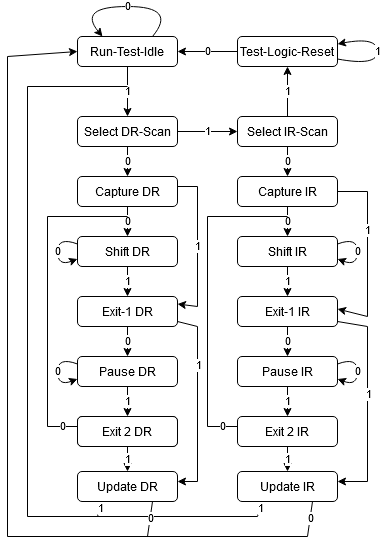
\includegraphics[width= 0.35 \textwidth]{figures/jtagstatemachine.png}
\caption{JTAG state machine. On each rising edge of TCK, the state machine progresses to a new state by checking the value of TMS.}
\label{fig:jtagstatemachine}
\end{figure}

\begin{figure}[H]
\centering
\resizebox{\textwidth}{!}{
\begin{tabular}{|l|l|} \hline
 Opcode (Decimal)& Function\\ \hline
   0     & No Op \\
   1     & JTAG System Reset (JTAG\_SYS\_RST), Equivalent to power on reset without reprogramming. \\
	       & Instruction only, (Auto reset) \\
   2     & DCFEB status reg (32 bits) shift only for reading back without updating \\
   3     & DCFEB status reg (32 bits) capture and shift for updated information. \\
   4     & Program Comparator DAC -- same as in old CFEB \\
   5     & Set Extra L1a Delay (2 bits) -- not used on DCFEB, exist for compatability with old DMB \\
   6     & Read FIFO 1 -- ADC data (16 channels x 12 bits = 192 bits) wide X (6 chips x 8 sample)/ \\
	       & event deep \\
   7     & Set F5, F8, and F9 in one serial loop (daisy chained) for compatability with old DMB \\
   8     & Set Pre Block End (4 bits) (not needed in DCFEB) -- not used on DCFEB, exist for \\
	       & compatability with old DMB \\
   9     & Set Comparator Mode and Timing (5 bits) same format as old CFEB \\
  10     & Set Buckeye Mask for shifting (6 bits) (default 6'b111111) same format as old CFEB, one \\
	       & bit for each chip \\
  11     & Shift data to/from Buckeye chips (48 bits/chip) \\
  12     & Set ADC configuration MASK (12 bits) \\
  13     & Command to initialize ADC -- Instruction only, (Auto reset) \\
  14     & Shift data and write to ADC configuration memory (26 bits) \\
  15     & Command to restart pipeline -- Instruction only, (Auto reset) \\
  16     & Set pipeline depth (9 bits) \\
  17     & Set TTC source (2 bits) Selects 0:FF\_EMU\_mode, 1:FF\_EEM\_mode, or 2:Skew\_Clr\_mode \\
  18     & Set calibration mode to external. (only for optical modes) -- Instruction only \\
  19     & Set calibration mode to internal. (only for optical modes) -- Instruction only \\
  20     & Set number of samples to readout (7 bits). \\
  21     & Write word to BPI interface write FIFO (16 bits). \\
  22     & Read word from BPI readback FIFO (16 bits). \\
  23     & Read status word from BPI interface (16 bits). \\
  24     & Read BPI timer (32 bits). \\
  25     & Reset BPI interface. -- Instruction only, (Auto reset) \\
  26     & Disable BPI processing. -- Instruction only, persisting \\
  27     & Enable BPI processing. -- Instruction only, persisting \\
  28     & Comparator Clock phase register (5-bits, 0-31). \\
  29     & TMB transmit mode (2-bits, 0: comparator data, 1: fixed patterns, 2: counters, 3: \\
	       & randoms, 4: comparator data, 5: half strip patterns). \\
  30     & TMB half strips for injecting patterns into the optical serial data stream for transmit \\
	       & mode 5. (30-bits, 5 per layer) {ly6,...ly1} \\
  31     & TMB layer mask to indicat the active layers for half strip patterns in transmit mode 5. \\
	       & (6-bits, 1 per layer) \\
  32     & Set DAQ rate to 1 GbE (1.25Gbps line rate) -- Instruction only \\
  33     & Set DAQ rate to 2.56 GbE (3.2Gbps line rate) -- Instruction only \\
  34     & Program Calibration DAC -- same style as Comparator DAC \\
  35     & Send Control Byte to the MAX 1271 ADC (and conversion clocks) \\
  36     & Read back the MAX 1271 ADC conversion stored in the SPI return register. \\
  37     & Read the SEM status (10 bits). \\
  38     & Reset the configuration ECC error counters. -- Instruction only, (Auto reset) \\
  39     & Read the ECC error counters (16-bits total, \{8-bits for multi-bit error count, 8-bits \\
	       & for single-bit error counts\}) \\
  40     & Set L1A\_MATCH source to use only matched L1A's (skw\_rw\_l1a\_match). Clear the \\
	       & USE\_ANY\_L1A flag. -- Instruction only \\
  41     & Set L1A\_MATCH source to use any L1A to send data (skw\_rw\_l1a). Set the USE\_ANY\_L1A flag \\
	       & -- Instruction only \\ \hline
\end{tabular}}
\caption{(x)DCFEB JTAG commands}
\label{tab:dcfebcommands1}
\end{figure}

\begin{figure}[H]
\centering
\resizebox{\textwidth}{!}{
\begin{tabular}{|l|l|} \hline
 Opcode (Decimal)& Function\\ \hline
  42     & Disable l1anum use in data to ODMB. Clear the L1A\_HEAD flag. -- Instruction only \\
  43     & Enable l1anum use in data to ODMB. Set the L1A\_HEAD flag.  This is the default \\
	       & -- Instruction only \\
  44     & Sampling Clock phase register (3-bits, 0-7). \\
  45     & PRBS test mode for DAQ optical path (3-bits, 0-7). \\
  46     & Inject error into PRBS test for DAQ optical path. \\
  47     & Take control of the SEM command interface (only needs to be set after ChipScope Pro has \\
	       & been in control). \\
  48     & Reset the double error detected flag (SEM module). \\
  49     & Send ASCII command to the SEM controller (8-bits). \\
  50     & Frame Address Register (FAR) in Linear Address format indicating the frame containing \\
	       & the error (24-bits). \\
  51     & Frame Address Register (FAR) in Physical Address format indicating the frame containing \\
	       & the error (24-bits). \\
  52     & Register Selection Word (Reg\_Sel\_Wrd) for selecting which register to independently \\
	       & capture and readback (8-bits). \\
  53     & Readback Select Register: Register to capture selected register indicated in \\
	       & Reg\_Sel\_Wrd (16-bits). \\
  54     & QPLL reset: This requires a NoOp afterwards to clear the reset then a Hard reset. All \\
	       & clocks stop while active. QPLL takes 0.5 seconds to lock. \\
  55     & QPLL lock lost counter (8-bits). \\
  56     & Startup Status register (16-bits).  \{qpll\_lock,qpll\_error,qpll\_cnt\_ovrflw,1'b0,eos, \\
	       & trg\_mmcm\_lock,daq\_mmcm\_lock,adc\_rdy,run,al\_status[2:0],por\_state[3:0]\}; \\
  57     & Read L1A counter (24 bits). \\
  58     & Read L1A\_MATCH counter (12 bits). \\
  59     & Read INJPLS counter (12 bits). \\
  60     & Read EXTPLS counter (12 bits). \\
  61     & Read BC0 counter (12 bits). \\
  62     & Comparator Clock Phase Reset (CMP\_PHS\_JTAG\_RST),  Instruction only, (Auto reset) \\
  63     & Toggle transmit disable on DAQ optical transceiver \\
  64     & Toggle transmit disable on TRG optical transceiver \\
  65     & Enable  ECC for parameters storage in XCF08P PROM Set   the ECC flag. -- Instruction \\
	       & only, persisting  This is the default \\
  66     & Disable ECC for parameters storage in XCF08P PROM Clear the ECC flag. -- Instruction \\
	       & only, persisting \\
  67     & Enable  CRC for parameters storage in XCF08P PROM Set   the CRC flag. -- Instruction \\
	       & only, persisting \\
  68     & Disable CRC for parameters storage in XCF08P PROM Clear the CRC flag. -- Instruction \\
	       & only, persisting  This is the default \\
  69     & Enable  ECC Decoding for parameters readback of XCF08P PROM Set   the DECODE flag. \\
	       & -- Instruction only, persisting  This is the default \\
  70     & Disable ECC Decoding for parameters readback of XCF08P PROM Clear the DECODE flag. \\
	       & -- Instruction only, persisting \\
  71     & Initiate transfer of parameters from XCF08P PROM to readback FIFO -- Instruction only, \\
	       & (Auto reset) \\
  72     & Read word from XCF08P PROM readback FIFO (16 bits). \\
  73     & Enable  GBT Testing mode -- Instruction only, persisting \\
  74     & Disable GBT Testing mode -- Instruction only, persisting  This is the default \\
  75     & Enable power to GBT -- Instruction only, persisting  This is the default \\ 
  76     & Disable power to GBT -- Instruction only, persisting \\
  77     & Write Byte to I2C write FIFO (8 bits). \\
  78     & Read Byte from I2C readback FIFO (8 bits). \\
  79     & Read I2C status word from I2C interface (8 bits). \\
  80     & Reset I2C interface. -- Instruction only, (Auto reset) \\
  81     & Start I2C processing. -- Instruction only, persisting until new command or processing \\
	       & completed \\ \hline
\end{tabular}}
\caption{(x)DCFEB JTAG commands}
\label{tab:dcfebcommands2}
\end{figure}

\section{General Notes on Hardware and Firmware}

In general, it best to use synchronous logic where ever possible as asynchronous logic is more prone to strange behavior and is more difficult to debug. In particular, it is useful to make all VHDL processes of the form

\begin{listing}
process_name : process(CLK)
begin
if rising_edge(CLK) then
  --internal logic here
end if;
end process;
\end{listing}

In this way, it is clearer how this should be implemented on the FPGA (flip-flop + LUT).

\section{ODMB Hardware}

\section{ODMB Firmware}

\subsection{Top Level}

The current ODMB firmware is largely split into two pieces The first is ODMB VME (MBV), which executes slow control such as sending commands to DCFEB or LVMB and changing ODMB settings. The second is ODMB CTRL (MBC), which executes fast control needed during data taking.

%\subsubsection{Clocks and QPLL}
The 160MHz and 40MHz clocks are produced by the qpll and are inputs to the FPGA. The \texttt{qpll\_reset} and \texttt{qpll\_autorestart} signals are held at `1'. The faster clocks (10 MHz, and 5 MHz) are then generated by a clock manager (MMCM) ip core from the 40 MHz clock. The slightly slower clocks (2.5 MHz, 5 MHz, 1.25 MHz, 0.625 MHz) are generated by dividing the 5 MHz clock with D flops. Finally, the very slow clocks (10 kHz and 1 kHz) are generated in a process with a counter.

%\subsubsection{VME Interface}
The VME interface consists of several signals, which go to the IC's on the ODMB that ultimately interface with the VME backplane. These signals are summarized in table~\ref{tab:odmbvme} with signals for the ICs between the FPGA and VME backplane listed below the double line. Inside the ODMB, most of these signals are sent to the \texttt{COMMAND\_MODULE} module in ODMB VME, which decodes the VME commands and send appropriate signals such as \texttt{STROBE}, \texttt{DEVICE}, and \texttt{COMMAND} to the ODMB VME devices. 

For more on VME protocol, see the section on the VME simulation. For more information about how ODMB deals with VME commands, reference the section on command modules. 

\begin{table}[H]
\centering
\begin{tabular}{|l|l|} \hline
Port& Description\\ \hline
\texttt{vme\_data}& VME data IO line, IOBUF controlled by \texttt{vme\_tovme (bar)}.\\ \hline
\texttt{vme\_addr}& Address from VME, given to \texttt{COMMAND\_MODULE}. The first 5 bits specify \\
                  & the slot(s) being addressed and the later 18 bits define the command given.\\ \hline
\texttt{vme\_am}& Address modifier from VME, given to \texttt{COMMAND\_MODULE}. This specifies\\ 
                & the type of command being sent. \\ \hline
\texttt{vme\_gap}& Geographical address parity from VME, given to \texttt{COMMAND\_MODULE}. This \\
                & bit is 1 if \texttt{vme\_ga} has an even number of 1's and 0 otherwise. \\ \hline
\texttt{vme\_ga}& Geographical address from VME, given to \texttt{COMMAND\_MODULE}. These bits \\
                 & define the VME slot the board is currently connected to.\\ \hline
\texttt{vme\_as\_b}& Address strobe (bar) from VME, given to \texttt{COMMAND\_MODULE} and  \\
                   & \texttt{VMECONFREGS}. This signal can be asserted after \texttt{vme\_addr} is \\
									 & ready to be read.\\ \hline
\texttt{vme\_ds\_b}& Data strobe (bar) from VME, given to \texttt{COMMAND\_MODULE}. These signals \\
                   & can be asserted after \texttt{vme\_data} is ready to be read or VCC is ready \\
									 & to read data. Each one corresponds to one byte on \texttt{vme\_data}\\ \hline
\texttt{vme\_sysfail\_b}& Sysfail (bar) signal from VME, given to \texttt{COMMAND\_MODULE}. \\
                        & Indicates a failure of the VME system.\\ \hline
\texttt{vme\_berr\_b}& Error (bar) signal from VME, given to \texttt{COMMAND\_MODULE}. Indicates \\
                     & an error in VME system and postpones any commands.\\ \hline
\texttt{vme\_iack\_b}& Interrupt acknowledge from VME, given to \texttt{COMMAND\_MODULE}. Commands \\
                     & should only be accepted while \texttt{IACK} is high, allowing VCC to \\
										 & interrupt commands by driving it low.\\ \hline
\texttt{vme\_lword\_b}& Load word signal from VME, given to \texttt{COMMAND\_MODULE}. Defines size \\ 
                      & of data transfers.\\ \hline
\texttt{vme\_write\_b}& write (bar) signal from VME, given to each device in \texttt{ODMB VME}. \\
                      & Indicates if the current command is a read or write command.\\ \hline
\texttt{vme\_dtack\_v6\_b}& Data acknowledge (bar) signal to VME, low when any \\
                 & device from ODMB VME issues a dtack.\\ \hline \hline
\texttt{vme\_tovme}& Output signal controlling direction of \texttt{vme\_data} both internally and \\
          & on level translator ICs. Not of \texttt{tovme\_b} from \texttt{COMMAND\_MODULE}\\ \hline
\texttt{vme\_doe\_b}& VME output enable (bar) signal from \texttt{COMMAND\_MODULE} for level \\
                    & translator ICs.\\ \hline
\end{tabular}
\caption{Signals in VME interface}
\label{tab:odmbvme}
\end{table}

\subsection{ODMB VME: Command Module}

The command module (command.vhd) is a helper device in the ODMB VME interface responsible for decoding the signals received from the VME backplane. The signals connecting to this interface are listed in table \ref{tab:commandinterface}.

\begin{table}[H]
\centering
\begin{tabular}{|l|l|} \hline
Port& Description\\ \hline
\texttt{FASTCLK}& 40MHz clock from top level\\ \hline
\texttt{SLOWCLK}& 2.5MHz clock from top level\\ \hline
\texttt{GA}& VME geographical address from \texttt{VME\_GA} and \texttt{VME\_GAP} (\texttt{GA(5)} should be \texttt{VME\_GAP})\\ \hline
\texttt{ADR}& VME address from \texttt{VME\_ADDR}\\ \hline
\texttt{AM}& VME address modifier from \texttt{VME\_AM}\\ \hline
\texttt{AS}& VME address strobe (bar) from \texttt{VME\_AS\_B}\\ \hline
\texttt{DS0}& Lower bit of VME data strobe (bar) from \texttt{VME\_DS\_B(0)}\\ \hline
\texttt{DS1}& Upper bit of VME data strobe (bar) from \texttt{VME\_DS\_B(1)}\\ \hline
\texttt{LWORD}& VME load word (bar) from \texttt{VME\_LWORD\_B}\\ \hline
\texttt{WRITER}& VME write (bar) signal from \texttt{VME\_WRITE\_B}\\ \hline
\texttt{IACK}& VME interrupt acknowledge (bar) from \texttt{VME\_IACK\_B}\\ \hline
\texttt{BERR}& VME error (bar) signal from \texttt{VME\_BERR\_B}\\ \hline
\texttt{SYSFAIL}& VME SYSFAIL (bar) signal from \texttt{VME\_SYSFAIL\_B}\\ \hline
\texttt{TOVME\_B}& signal controlling \texttt{VME\_DATA} IOBUF at top level and output as (barred) \texttt{VME\_TOVME}\\ \hline
\texttt{DOE\_B}& VME output enable (bar) output as \texttt{VME\_DOE\_B}\\ \hline
\texttt{DEVICE}& each of 10 bits indicates to ODMB VME device if it is selected\\ \hline
\texttt{STROBE}& signal sent to ODMB VME devices to indicate command ready\\ \hline
\texttt{COMMAND}& decoded VME command sent to each ODMB VME device\\ \hline
\texttt{ADRS}& used to multiplex \texttt{VME\_DATA\_OUT} from the various devices\\ \hline
\texttt{DIAGOUT}& for debugging\\ \hline
\texttt{LED}& for debugging\\ \hline
\end{tabular}
\caption{Signals in command module device}
\label{tab:commandinterface}
\end{table}

This device records the values of \texttt{AM} and \texttt{ADDR} (as \texttt{AMS} and \texttt{ADDR\_INNER} as they are when \texttt{AS} goes low (when \texttt{AS} is high, the internal values directly reflect the current values provided by the VME backplane). The command module interprets these to generate \texttt{DEVICE} and \texttt{COMMAND}, which are sent to the ODMB VME modules to interpret.

The command module checks that \texttt{GAP} matches the parity of the number of zeroes of \texttt{GA} and saves the result as \texttt{VALIDGA/GOODGA}. It checks AMS, and the ODMB only responds to commands with the format ``111XYZ'' where Y$\neq$Z and for which LWORD is 1. It also checks for commands it should respond to, which either (1) are addressed to this particular slot and have \texttt{ADDR}(23 downto 19) matching \texttt{GA}, (2) are broadcasted and have \texttt{ADDR}(23 downto 19) as ``11111'', or (3) \texttt{GA} is ``00000'', which indicates the \texttt{GA} pins are not functional. If the ODMB should respond to a particular commnad, \texttt{BOARDENB} is set high. Finally, this module checks \texttt{SYSFAIL} and \texttt{IACK}, which should both be high for the ODMB to respond to a command. When \texttt{GAP} is valid, \texttt{AM} and \texttt{LWORD} are appropriate, the command is for the ODMB, and no failures or interrupts are detected, the command module assigns \texttt{tovme} based on \texttt{write}. When the above conditions are met and both \texttt{DS0} and \texttt{DS1} are low, it generates the signal \texttt{strobe} and sends it to the ODMB VME modules to prompt action.

\subsection{VME Device 1: DCFEB JTAG and INITJAG}

The DCFEB JTAG device (cfebjtag.vhd) is the first device in the ODMB VME interface. This module is used to communicate with (x)(D)CFEBs via JTAG protocol (via the PPIB skew clear cables). The signals connecting to this interface are listed in table \ref{tab:cfebjtaginterface}. The VME command recognized by this device are shown in table \ref{tab:cfebjtagcommands}.

\begin{table}[H]
\centering
\begin{tabular}{|l|l|} \hline
Port& Description\\ \hline
\texttt{FASTCLK}& 40MHz clock from top level\\ \hline
\texttt{SLOWCLK}& 2.5MHz clock from top level. Called \texttt{clk\_s1} in odmb\_vme.vhd and top level \\ \hline
\texttt{RST}& Reset signal.\\ \hline
\texttt{DEVICE}& Signal to accept/ignore incoming commands/strobes. Should be connected to  \\
      & DEVICE(1) output from \texttt{COMMAND\_MODULE}, which decodes VME commands- will  \\
			& be 1 for VME commands \texttt{1XXX}.\\ \hline 
\texttt{STROBE}& Signal that initiates command execution; generated by \texttt{COMMAND\_MODULE} \\
      & from VME strobe signals\\ \hline
\texttt{COMMAND}& Important bits of VME command (append ``00'' to end for full command)\\ \hline
\texttt{WRITER}& Unused, connected from \texttt{VME\_WRITE\_B}\\ \hline
\texttt{INDATA}& input directly from \texttt{VME\_DATA} line (through IOBUF)\\ \hline
\texttt{OUTDATA}& output multiplexed to \texttt{VME\_DATA} line (through IOBUF)\\ \hline
\texttt{DTACK}& acknowledge receipt of VME commands, NOR'd with DTACKs from other devices \\
     & and sent back to VME. Active high.\\ \hline
\texttt{INITJTAGS}& signal that resets module and sends signals to reset CFEB JTAG \\
         & state machine, generated when DONE received from (x)(D)CFEBs\\ \hline
\texttt{TCK}& JTAG output to (x)(D)CFEB, one per (x)(D)CFEB\\ \hline
\texttt{TDI}& JTAG output to (x)(D)CFEB, common to all (x)(D)CFEBs\\ \hline
\texttt{TMS}& JTAG output to (x)(D)CFEB, common to all (x)(D)CFEBs\\ \hline
\texttt{FEBTDO}& JTAG input from (x)(D)CFEB, one per (x)(D)CFEBs\\ \hline
\texttt{LED}& DEBUG output\\ \hline
\texttt{DIAGOUT}& DEBUG output\\ \hline
\end{tabular}
\caption{Ports for CFEBJTAG device}
\label{tab:cfebjtaginterface}
\end{table}

\begin{table}[H]
\centering
\begin{tabular}{|l|l|} \hline
COMMAND& Description\\ \hline
\texttt{W 1Y00}& Shift data, no TMS header or tailer.\\ \hline
\texttt{W 1Y04}& Shift data, preceded by TMS header.\\ \hline
\texttt{W 1Y08}& Shift data, followed by TMS tailer.\\ \hline
\texttt{W 1Y0C}& Shift data, preceded by TMS header and followed by TMS tailer.\\ \hline
\texttt{R 1014}& Read TDO register.\\ \hline
\texttt{W 1018}& Reset JTAG to idle.\\ \hline
\texttt{W 1Y1C}& Shift data, preceded by TMS header and followed by TMS tailer. (Legacy)\\ \hline
\texttt{W 1020}& Select DCFEB (1 bit per DCFEB).\\ \hline
\texttt{R 1024}& Read selected DCFEBs.\\ \hline
\texttt{W 1Y30}& Shift instruction, no TMS header or tailer.\\ \hline
\texttt{W 1Y34}& Shift instruction, preceded by TMS header.\\ \hline
\texttt{W 1Y38}& Shift instruction, followed by TMS tailer.\\ \hline
\texttt{W 1Y3C}& Shift instruction, preceded by TMS header and followed by TMS tailer.\\ \hline
\texttt{W 1Y48}& Shift instruction, followed by special TMS tailer.\\ \hline
\texttt{W 1Y4C}& Shift instruction, preceded by TMS header and followed by special TMS tailer.\\ \hline
\end{tabular}
\caption{CFEB JTAG accepted commands}
\label{tab:cfebjtagcommands}
\end{table}

%command interpretation
The CFEBJTAG module continuously interprets \texttt{COMMAND}, which is loaded from \texttt{VME\_ADDR} by the command module upon receiving an address strobe. There are two general classes of commands, data shift and instruction shift commands, as well as four special case commands: read TDO, reset JTAG, select DCFEB, and read selected DCFEB. Upon receiving a strobe signal, actions are executed depending on the current command.

%special commands, except for reset jtag
The special commands are each handled by their own block of VHDL. The read TDO command simply presents the last 16 bits read from TDO during data or instruction shifts and presents a DTACK signal. Note that the last 16 bits may not have come from the same shift commands, if the shift commands were less than the maximum 16 bits. The select DCFEB command sets the \texttt{selfeb} registers, which control which DCFEBs are addressed when shift commands are issued, and presents a DTACK signal. Note that when a reset JTAG command is issued or the \texttt{INITJTAGS} signal is received, all of the DCFEBs are automatically selected to broadcast the reset pattern. The read selected DCFEB command simply outputs the contents of the \texttt{selfeb} registers and presents a DTACK signal. The reset JTAG command sends a TMS pattern (111110) to all DCFEBs and functions similarly to shift commands detailed below. The reset JTAG command is also automatically executed when the \texttt{INITJTAGS} signal is received.

%TCK generation
The JTAG protocol signals output by CFEBJTAG are TCK, TMS, and TDI while TDO is an input. These are used for all shift commands as well as by the reset JTAG command. When a strobe initiates a shift command, a signal called \texttt{load} is pulsed. This in turns causes \texttt{busy} to go high. If a new strobe signal arrives, the module waits until \texttt{busy} is de-asserted before asserting load again. While \texttt{busy} is asserted or a reset JTAG command is being executed, the \text{global\_tck} clock will run at half the frequency of \texttt{SLOWCLK} (1.25 MHz). This is sent to the \texttt{TCK} specific to each DCFEB if that particular DCFEB is selected.

%TMS generation
There are several separate blocks of VHDL that handle generation of TMS patterns, but they all have roughly the same structure. First, there is an enable section that checks if the TMS pattern in question should be enabled based on the type of command issued and what has already been transmitted. For example, the tailer enable checks if the current instruction requires a tailer and if the data
section has already finished. Next, there is a done section, which simply uses a counter to set a done register after the appropriate number of clock cycles, noting again that TCK runs at half the speed of \texttt{SLOWCLK}. Finally, the actual TMS patterns are generated by a loop of flip-flops connected end to end. The desired sequence of 1's and 0's are set by using FDP(E) and FDC(E) flip flops and due to the looping nature of the connection, the pattern returns to its original state after a full transmission. The sequence is shifted on each edge of \texttt{SLOWCLK} associated with a falling edge of the TCK clock. The 5 TMS blocks constructed in this way are the reset JTAG block (TMS pattern 111110), the data header block (TMS pattern 100), the instruction header block (TMS pattern 1100), the data block (TMS pattern is $n-1$ 0's followed by a 1 where $n$ is the length of the data being shifted), and the tailer block (TMS pattern 10, or just 1 for the special tailer).

Note the FD flops from the \texttt{Latches\_Flipflops} package are found not to work on the KCU105 evaluation board and were replaced with the equivalent UNISIM components. Furthermore, the CB4CE and SR16LCE functions from the \texttt{Latches\_Flipflops} package did not defaultly work on the KCU105 evaluation board, and their implementation was slightly tweaked to nest conditions rather than AND'ing them. It is unclear why this changes behavior.

%TDI and TDO
The TDI and TDO signals are more straightforward. When load is pulsed, \texttt{INDATA} is loaded into a 16 bit shift register with the lowest bit connected to TDI. The register is then cycled on edges of \texttt{SLOWCLK} corresponding to falling edges of TCK. TDO is sent to a similar shift register, where the bits are used to build \texttt{OUTDATA} that can then be read with the appropriate command.

%DTACK
Because no data is being presented to the VME, DTACK signals from reset JTAG or shift commands are simply presented a preset number of clock cycles after strobe is received.

%\subsubsection{DCFEB done in top level}
The \texttt{INITJTAG} signal is generated after receiving DONE from the (x)(D)CFEBs. The signal \texttt{pon\_rst\_reg} is initialized to a particular value when \texttt{PLL\_LOCK} is on (when ODMB is reset) and after a few clock cycles, \texttt{pon\_reset} becomes '1', which sets the FSM \texttt{done\_current\_state} to \texttt{DONE\_LOW}. When the \texttt{DONE} for an (x)(D)CFEB becomes `1', the \texttt{done\_current\_state} is set to \texttt{DONE\_COUNTING}, which generates \texttt{dcfeb\_done\_pulse} before setting the FSM to \texttt{DONE\_IDLE}. All the \texttt{dcfeb\_done\_pulse}'s are OR'd together and converted to a pulse to generate \texttt{INITJTAG}. Perhaps this logic could be moved from the top level to inside of cfebjtag.vhd. Note that the FSM counter runs on the 10 kHz clock, which is just generated in a process somewhere and not BUFG'd. 

\subsection{VME Device 3: VMEMON}

The VMEMON device (vmemon.vhd) also known as ODMB/DCFEB control is the third device in the ODMB VME interface. This module is used to set various configuration registers and read back various data registers. The signals connecting to this interface are listed in table \ref{tab:vmemoninterface}.

\begin{table}[H]
\centering
\begin{tabular}{|l|l|} \hline
Port& Description\\ \hline
\texttt{CLK40}& 40MHz clock from top level\\ \hline
\texttt{SLOWCLK}& 2.5MHz clock from top level. Called \texttt{clk\_s1} in odmb\_vme.vhd and top level. \\ \hline
\texttt{RST}& Reset signal.\\ \hline
\texttt{DEVICE}& Signal to accept/ignore incoming commands/strobes. Should be connected to \\
      & DEVICE(3) output from \texttt{COMMAND\_MODULE}, which decodes VME commands- will be 1 \\
			& for VME commands 3XXX.\\ \hline 
\texttt{STROBE}& Signal that initiates command execution; generated by \texttt{COMMAND\_MODULE} \\
      & from VME strobe signals\\ \hline
\texttt{COMMAND}& Important bits of VME command (append ``00'' to end for full command)\\ \hline
\texttt{WRITER}& Indicates direction of read/write commands, connected from \texttt{VME\_WRITE\_B}\\ \hline
\texttt{INDATA}& input directly from \texttt{VME\_DATA} line (through IOBUF)\\ \hline
\texttt{OUTDATA}& output multiplexed to \texttt{VME\_DATA} line (through IOBUF)\\ \hline
\texttt{DTACK}& acknowledge receipt of VME commands, OR'd with DTACKs from other devices \\
     & and sent back to VME. Active high\\ \hline
\texttt{DCFEB\_DONE}& Vector of \texttt{DONE} signals directly from PPIB.\\ \hline
\texttt{QPLL\_LOCKED}& QPLL lock signal directly from QPLL.\\ \hline
\texttt{OPT\_RESET\_PULSE}& output signal that generates a pulse in the reset signal to the \\
                          & GTX/GTH modules.\\ \hline
\texttt{L1A\_RESET\_PULSE}& output signal that generates a reset signal to the L1A counter\\
                          & (in ODMB CTRL) and CFEB RESYNC.\\ \hline
\texttt{FW\_RESET}& output signal that generates a general soft reset (to ODMB CTRL, BPI \\
                  & interface, etc.).\\ \hline
\texttt{REPROG\_B}& output hard reset output signal to CFEBs.\\ \hline
\texttt{TEST\_INJ}& output sent to \texttt{TEST\_CCBINJ} port of ODMB CTRL to generate INJPLSes. \\ \hline
\texttt{TEST\_PLS}& output sent to \texttt{TEST\_CCBPLS} port of ODMB CTRL to generate EXTPLSes. \\ \hline
\texttt{TEST\_PED}& output sent to \texttt{TEST\_CCBPED} port of ODMB CTRL. \\ \hline
\texttt{TEST\_BC0}& output sent to PPIB (output \texttt{DCFEB\_BC0}) after delay. \\ \hline
\texttt{TEST\_LCT}& output that generates an L1A in the top level. \\ \hline
\texttt{OTMB\_LCT\_RQST}& output sent to OTMB (output \texttt{LCTRQST}(1)) \\ \hline
\texttt{OTMB\_EXT\_TRIG}& output sent to OTMB (output \texttt{LCTRQST}(2)) \\ \hline
\texttt{MASK\_PLS}& output masks to '0' signal from ODMB CTRL to DCFEB pulses (output \\ 
                  & \texttt{DCFEB\_INJPLS} and \texttt{DCFEB\_EXTPLS}) \\ \hline
\texttt{MASK\_L1A}& output masks to '0' DCFEB-bound signals \texttt{DCFEB\_L1A} and \\
                  & \texttt{DCFEB\_L1A\_MATCH} \\ \hline
\texttt{MASK\_L1A}& output masks to '0' DCFEB-bound signals \texttt{DCFEB\_L1A} and \\
                  & \texttt{DCFEB\_L1A\_MATCH} \\ \hline
\texttt{TP\_SEL}& output that selects what signals are on which test ODMB points \\ \hline
\texttt{MAX\_WORDS\_DCFEB}& output that sets number of invalid words received from a DCFEB before \\
                          & it is considered bad\\ \hline
\texttt{ODMB\_CTRL}& output, control bits for ODMB, see Table~\ref{tab:odmbctrlbits}. Split in ODMB7.\\ \hline
\texttt{ODMB\_DATA\_SEL}& output, selects configuration data to read from top level, see manual.\\ \hline
\texttt{ODMB\_DATA}& input from top level with configuration data to read\\ \hline
\texttt{TXDIFFCTRL}& output signal that controls voltage swings on the GTX/GTH modules.\\ \hline
\texttt{LOOPBACK}& output signal to GTX/GTH modules needed for loopback tests.\\ \hline
\end{tabular}
\caption{Ports for VMEMON device}
\label{tab:vmemoninterface}
\end{table}

\begin{table}[H]
\centering
\begin{tabular}{|l|l|l|} \hline
Bits& ODMB7 Port& Description\\ \hline
5 downto 0& \texttt{ODMB\_CAL}& calibration mode, sent to ODMB CTRL (1: generate L1A with each pulse)\\ \hline
6& -& Unused \\ \hline
7& \texttt{MUX\_DATA\_PATH}& data multiplexer (0: real data from ALCT/DCFEB/OTMB, 1: dummy data)\\ \hline
8& -& ODMB soft reset, only used for reference\\ \hline
9& \texttt{MUX\_TRIGGER}& trigger multiplexer, used various places (0: external triggers, 1: internal triggers)\\ \hline 
10& \texttt{MUX\_LVMB}& LVMB multiplexer, sent to LVMB\_MUX module (0: real LVMB, 1: dummy LVMB)\\ \hline
11& -& Mask L1A's/L1A Matches, only used for reference \\ \hline
12& -& Mask L1A's/L1A Matches, only used for reference \\ \hline
13& \texttt{ODMB\_PED}&  Pedestal mode, sent to ODMB CTRL (1: L1A\_MATCH sent with each L1A)\\ \hline 
14& \texttt{ODMB\_PED}&  OTMB Pedestal mode, sent to ODMB CTRL (1: L1A\_MATCH sent with each L1A)\\ \hline
15& -& Unused \\ \hline	
\end{tabular}
\caption{Bits in \texttt{ODMB\_CTRL\_REG}}
\label{tab:odmbctrlbits}
\end{table}

\begin{table}[H]
\centering
\begin{tabular}{|l|l|} \hline
COMMAND& Description\\ \hline
\texttt{W/R 3000}& Set or read mode. 0 = nominal mode, 1 = calibration mode (L1A with each pulse).\\ \hline
\texttt{W 3004}& ODMB Soft reset.\\ \hline
\texttt{W 3008}& ODMB Optical reset.\\ \hline
\texttt{W 3010}& Reprogram all DCFEBs.\\ \hline
\texttt{R 3014}& L1A reset and DCFEB resync.\\ \hline
\texttt{W/R 3020}& Set or read \texttt{TP\_SEL} (controls signals sent to test points).\\ \hline
\texttt{W/R 3024}& Set or read number of words in DCFEB packet before autokill. Default 1024.\\ \hline
\texttt{W/R 3100}& Set or read loopback. 0 = no loopback, 1/2 = internal loopback.\\ \hline
\texttt{R 3110}& Read \text{DIFFCTRL} (TX voltage swing). 0 = min($\sim$100 mV), F = max($\sim$1100 mV).\\ \hline
\texttt{R 3120}& Read DONE bits from DCFEBs.\\ \hline
\texttt{R 3124}& Read QPLL lock.\\ \hline
\texttt{W 3200}& Send pulses to DCFEBs, see Table~\ref{tab:dcfebpulses}.\\ \hline
\texttt{W/R 3300}& Set or read data MUX. 0 = real data, 1 = dummy data.\\ \hline
\texttt{W/R 3304}& Set or read trigger MUX. 0 = external triggers, 1 = internal triggers.\\ \hline
\texttt{W/R 3308}& Set or read LVMB MUX. 0 = real LVMB, 1 = dummy LVMB.\\ \hline
\texttt{W/R 3400}& Set or read pedestal mode. 0 = normal, 1 = \texttt{L1A\_MATCH} to DCFEB for each \texttt{L1A}. \\ \hline
\texttt{W/R 3404}& Set or read OTMB pedestal. 0 = normal, 1 = data request to OTMB for each \texttt{L1A}.\\ \hline
\texttt{W/R 3408}& Set or read \texttt{L1A} mask. Bit 0 kills \texttt{L1A}s bits 1-7 kill \texttt{L1A\_MATCHES}.\\ \hline
\texttt{W/R 340C}& Set or read \texttt{MASK\_PLS}. 0 = normal, 1 = no \texttt{EXT/INJPLS} from CCB.\\ \hline
\texttt{R 3YZC}& Read data, see Table~\ref{tab:readdata}.\\ \hline 
\end{tabular}
\caption{VMEMON accepted commands}
\label{tab:vmemoncommands}
\end{table}

\begin{table}[H]
\centering
\begin{tabular}{|l|l|} \hline
Bits&  Description\\ \hline
0& Sends \texttt{INJPLS} (port \texttt{TEST\_INJ}) to all DCFEBs\\ \hline
1& Sends \texttt{EXTPLS} (port \texttt{TEST\_PLS}) to all DCFEBs\\ \hline
2& Sends \texttt{L1A} and \texttt{L1A\_MATCH} (port \texttt{TEST\_LCT}) to non-killed DCFEBs\\ \hline
3& Sends LCT request (port \texttt{OTMB\_LCT\_RQST}) to OTMB\\ \hline
4& Sends external trigger request (port \texttt{OTMB\_EXT\_TRIG}) to OTMB\\ \hline
5& Sends \texttt{BC0} (port \texttt{TEST\_BC0}) to all DCFEBs\\ \hline	
\end{tabular}
\caption{Bits in \texttt{ODMB\_CTRL\_REG}}
\label{tab:dcfebpulses}
\end{table}

\begin{table}[H]
\centering
\begin{tabular}{|l|l|} \hline
\texttt{vme\_addr}(11 downto 4)&  Description\\ \hline
00& \texttt{odmb\_status}\\ \hline
01& \texttt{odmb\_ctrl}, see Table~\ref{tab:odmbctrlbits}\\ \hline
02-1F& Reserved for debugging purposes\\ \hline
20& \texttt{vme\_ga} and \texttt{vme\_gap}\\ \hline
21-29& \texttt{l1a\_match\_cnt} 1 through 9\\ \hline
2A& \texttt{alct\_push\_dly}\\ \hline
2B& \texttt{otmb\_push\_dly}\\ \hline
2C& \texttt{push\_dly}\\ \hline
2D& \texttt{lct\_l1a\_dly}\\ \hline
31-37& gap in BXs between last LCT and L1A for DCFEB 1-7\\ \hline
38& gap in BXs between last L1A and OTMBDAV\\ \hline
39& gap in BXs between last L1A and ALCTDAV\\ \hline
3A-3B& CAFIFO L1A counter upper and lower bits\\ \hline
3C& CAFIFO BX count\\ \hline
3D& CAFIFO read and write addresses\\ \hline
3E& \texttt{cafifo\_l1a\_match\_in}\\ \hline
3F& L1A counter\\ \hline
41-49& Number packets received for DCFEBs, OTMB, or ALCT\\ \hline
4A& Number packets sent to DDU\\ \hline
4B& Number packets sent to PC\\ \hline
4D& \texttt{cafifo\_l1a\_match\_out}\\ \hline
4E& \texttt{cafifo\_l1a\_dav}\\ \hline
4F& QPLL Locked Counter\\ \hline
51-59& Number packets sent to DDU for DCFEBs, OTMB, or ALCT\\ \hline
5A& Last \texttt{ccb\_cmd}, \texttt{evtrst}, \texttt{bxrst}\\ \hline
5B& Last \texttt{ccb\_data} strobed\\ \hline
5C& Misc CCB registers: \texttt{ccb\_cal}+\texttt{ccb\_bx0}+\texttt{ccb\_bxrst}\\
  & +\texttt{ccb\_l1arst}+\texttt{ccb\_l1a}+\texttt{ccb\_clken}+\texttt{ccb\_evtrst}\\
	& +\texttt{ccb\_cmd\_strobe}+\texttt{ccb\_data\_strobe}\\ \hline
5D& \texttt{ccb\_rsv\_reg}\\ \hline
5F& L1A counter ignoring resyncs\\ \hline
61-67& Number packets with good CRCs for each DCFEB\\ \hline
71-77& Raw LCT counters for each DCFEB\\ \hline
78& OTMB DAV counter\\ \hline
79& ALCT DAV counter\\ \hline
81-89& Number fully arrived packets for DCFEBs, OTMB, and ALCT\\ \hline
91-99& Times cafifo data was available for DCFEBs, OTMB, and ALCT\\ \hline
A1-A7& Number packets with bad CRCs for each DCFEB\\ \hline
A8& Times DDU TX PLL lost its lock\\ \hline
A9& Times DDU RX has erred\\ \hline
AA& Number bit errors in DDU RX\\ \hline
AB& Times PC RX has erred\\ \hline
AC& Number bit errors in PC RX\\ \hline
B1-B7& Number fiber errors for DCFEB RX in last 63 cc\\ \hline
B8& DCFEBs auto-killed\\ \hline
B9& DCFEBs auto-killed due to fiber errors\\ \hline
\end{tabular}
\caption{Data accessible with command 0x3YZC}
\label{tab:readdata}
\end{table}

Roughly speaking, the four types of commands accepted by the VMEMON device are reset commands, internal register read/write commands, pulse commands, and the external ODMB data read command, as detailed in table~\ref{tab:vmemoncommands}. The reset commands are used to pulse various reset signals using the \texttt{PULSE2FAST} module for ODMB reset, L1A reset, and optical reset, and the \texttt{NPULSE2SAME} module for DCFEB reprogram. The internal register read/write commands store the VME input on a flip flop on write commands; the contents of the flip-flop are sent out of the module for use elsewhere in the ODMB firmware and can also be read out with the read commands. Note that the DCFEB done bits and the QPLL lock (in the ODMB 2013s) are treated in a similar manner despite being external signals and thus not writable. The pulse commands specified in table~\ref{tab:dcfebpulses} send out configuration pulses again using the \texttt{PULSE2FAST} and \texttt{NPULSE2SAME}. Finally, the ODMB data read command functions by setting the port \texttt{ODMB\_DATA\_SEL} based on the received command and outputting what is returned on the \texttt{ODMB\_DATA} port. The logic that assigns \texttt{ODMB\_DATA} based on \texttt{ODMB\_DATA\_SEL} is located in the ODMB top level file.

\subsection{VME Device 4: VMECONFREGS (Configuration Registers)}

\begin{table}[H]
\centering
\begin{tabular}{|l|l|} \hline
Port& Description\\ \hline
\texttt{CLK40}& 40MHz clock from top level.\\ \hline
\texttt{CLK}& 2.5MHz clock from top level.\\ \hline
\texttt{RST}& Reset signal.\\ \hline
\texttt{DEVICE}& Signal to accept/ignore incoming commands/strobes. Should be connected to \\
      & DEVICE(4) output from \texttt{COMMAND\_MODULE}, which decodes VME commands- will  \\
			& be 1 for VME commands 4XXX.\\ \hline 
\texttt{STROBE}& Signal that initiates command execution; generated by \\
      & \texttt{COMMAND\_MODULE} from VME strobe signals\\ \hline
\texttt{COMMAND}& Important bits of VME command (append ``00'' to end for full command)\\ \hline
\texttt{WRITER}& Indicates direction of read/write commands, connected from \\
               & \texttt{VME\_WRITE\_B}\\ \hline
\texttt{VME\_AS\_B}& VME address strobe, checked when from \texttt{VME\_AS\_B} (why?)\\ \hline
\texttt{INDATA}& input directly from \texttt{VME\_DATA} line (through IOBUF)\\ \hline
\texttt{OUTDATA}& output multiplexed to \texttt{VME\_DATA} line (through IOBUF)\\ \hline
\texttt{LCT\_L1A\_DLY}& outputs LCT L1A delay register (delays CLCT), used in ODMB CTRL\\
                      & and triggers. \\ \hline
\texttt{CABLE\_DLY}& outputs ALCT push delay register, used to delay L1A(\_MATCH)s, BC0s, \\
                   & and RESYNCs to DCFEBs\\ \hline
\texttt{OTMB\_PUSH\_DLY}& outputs OTMB push delay register (\texttt{OTMBDAV} is delayed by\\
                        & \texttt{push\_delay}-\texttt{OTMB\_PUSH\_DLY}), used in ODMB \\
												& CTRL and triggers\\ \hline
\texttt{ALCT\_PUSH\_DLY}& outputs ALCT push delay register (\texttt{ALCTDAV} is delayed by  \\
                        & \texttt{push\_delay}-\texttt{ALCT\_PUSH\_DLY}), used in ODMB \\
												& CTRL and triggers\\ \hline
\texttt{BX\_DLY}& outputs bunch crossing delay register, used in ODMB CTRL\\ \hline
\texttt{INJ\_DLY}& outputs INJ pulse delay register (delay from CCB calibration 1 pulse \\
                 & to DCFEB INJ pulse), used in ODMB CTRL\\ \hline
\texttt{EXT\_DLY}& outputs EXT pulse delay register (delay from CCB calibration 2 pulse \\
                 & to DCFEB EXT pulse), used in ODMB CTRL\\ \hline
\texttt{CALLCT\_DLY}& outputs CALLCT pulse delay register (delay from DCFEB INJ/EXT pulse \\
                 & to L1A), used in ODMB CTRL\\ \hline
\texttt{ODMB\_ID}& outputs ODMB unique ID from TMR const registers loaded from PROM, used \\
                 & by LVDBMON, ODMBJTAG, and DCFEB I/O to change behavior for different \\
								 & ODMB boards \\ \hline
\texttt{NWORDS\_DUMMY}& outputs number of words to generate to fake DCFEB and OTMB/ALCT\\ \hline
\texttt{KILL}& outputs whether to kill DCFEBs, ALCT, and OTMB, used various locations \\
             & including ODMB CTRL\\ \hline
\texttt{CRATEID}& outputs crate ID, used in ODMB CTRL when sending packets to DDU\\ \hline
\texttt{BPI\_CFG\_UL\_PULSE}& input from BPI\_PORT, indicates upload of CFG registers from\\
                            & PROM\\ \hline
\texttt{BPI\_CFG\_DL\_PULSE}& input from BPI\_PORT, indicates download of CFG registers \\
                            & to PROM (unused)\\ \hline
\texttt{BPI\_CONST\_UL\_PULSE}& input from BPI\_PORT, indicates upload of const registers \\
                              & from PROM\\ \hline
\texttt{BPI\_CONST\_DL\_PULSE}& input from BPI\_PORT, indicates download of const \\
                              & registers to PROM (unused)\\ \hline
\texttt{CHANGE\_REG\_DATA}& input from top level, contains current kill/bad DCFEBs\\ \hline
\texttt{CHANGE\_REG\_INDEX}& input from top level, is used to enable writing of KILL (7) \\
                           & and is 16 otherwise\\ \hline
\texttt{CC\_CFG\_REG\_IN}& input from BPI\_CTRL (PROM) used to load CFG and const \\
                         & registers\\ \hline
\texttt{BPI\_CONST\_BUSY}& input from BPI\_CONST\_CONTROLLER checked when writing to const \\
                         & registers\\ \hline
\texttt{CC\_CONST\_REG\_WE}& input from BPI\_CONST\_CONTROLLER checked when writing to \\
                           & const registers\\ \hline
\texttt{BPI\_CONST\_REGS}& output used to write to BPI\_CONST\_CONTROLLER\\ \hline
\texttt{BPI\_CFG\_BUSY}& input from BPI\_CFG\_CONTROLLER checked when writing to CFG\\
                       & registers\\ \hline
\texttt{CC\_CFG\_REG\_WE}& input from BPI\_CFG\_CONTROLLER checked when writing to CFG\\
                         & registers\\ \hline
\texttt{BPI\_CFG\_REGS}& output used to write to BPI\_CFG\_CONTROLLER\\ \hline
\end{tabular}
\caption{Ports on VMECONFREGS device}
\label{tab:vmeconfregsinterface}
\end{table}

The VMECONFREGS device is the fourth device in ODMB VME; its ports are shown in table~\ref{tab:vmeconfregsinterface}. This device deals with special configuration or CFG and protected or CONST registers. In the current firmware there are 16 CFG registers and 16 CONST registers, which are each 16 bits persistent across resets. The VMECONFREGS device accepts three classes of commands, each of which come in read and write varieties: read/write \texttt{mask\_vme}, read/write CFG registers, and read/write CONST registers.

The register \texttt{mask\_vme} allows or disallows writing to CONST registers via VME commands. Note that the separate \texttt{write\_const\_mask\_we} prevents writing to certain registers that are hardcoded in firmware, regardless of \texttt{mask\_vme}. This can be read and written with the 0x4FFC command.

The commands 0x40YZ allow for reading and writing of CFG registers. The CFG registers can also be written from PROM using the \texttt{BPI\_CFG\_UL\_PULSE} signals as well as by other parts of the ODMB firmware by setting \texttt{CHANGE\_REG\_INDEX} to the index of a particular CFG register. Currently, \texttt{CHANGE\_REG\_INDEX} is only used to set the KILL register (CFG register 7) when bad data is received from DCFEBs. Each CFG register is actually stored using triple modular redudancy (TMR) on 3 registers in the ODMB firmware. Each clock cycle these are updated by taking majority vote, so that if one register is changed, it will be restored on the next clock cycle. 

The 0x4Y00 commands where Y$\neq 0$ allow for reading and writing of the CONST registers. Similarly to the CFG registers, these can also be written from PROM using the \texttt{BPI\_CONST\_UL\_PULSE} signal. Note that CONST registers 1-4 (as well as CFG register 9) are hard-coded in the firmware and cannot be changed by the user or from PROM. Like CFG registers, the CONST registers also use TMR.

\subsection{ODMB CTRL Device 1: CALIBTRG}

This device generates calibration triggers when prompted by the CCB. It is used during STEP testing and calibration, but not during standard data taking. 

\begin{table}[H]
\centering
\begin{tabular}{|l|l|} \hline
Port& Description\\ \hline
\texttt{CMSCLK}& 40MHz clock input from top level\\ \hline
\texttt{CLK80}& 80MHz clock input from top level\\ \hline
\texttt{RST}& reset signal input from top level\\ \hline
\texttt{PLSINJEN}& pulse enable, input from ODMB CTRL, which just oscillates on and off when enabled\\ \hline
\texttt{CCBPLS}& input from ODMB CTRL to generate PLSBACK and INJPLS\\ \hline
\texttt{CCBINJ}& input from ODMB CTRL to generate INJBACK and INJPLS\\ \hline
\texttt{FINJ}& input from VMEMON to generate test INJBACK and INJPLS\\ \hline
\texttt{FPLS}& input from VMEMON to generate test PLSBACK and INJPLS\\ \hline
\texttt{FPED}& input from VMEMON to generate test pedestal output (unused)\\ \hline
\texttt{PRELCT}& input that generates PLS, tied to 0\\ \hline
\texttt{PREGTRG}& unused input, tied to 0\\ \hline
\texttt{INJ\_DLY}& input from VMECONFREGS indicating delay between CCB\_CAL1 and INJ\_PLS\\ \hline
\texttt{EXT\_DLY}& input from VMECONREGS indicating delay between CCB\_CAL0 and EXT\_PLS (PLSBACK)\\ \hline
\texttt{CALLCT\_DLY}& input from VMECONFREGS indicating delay between PLS and L1A\\ \hline
\texttt{LCT\_L1A\_DLY}& input from VMECONFREGS indicating delay between preLCT and L1A\\ \hline
\texttt{RNDMPLS}& unused input, tied to 0\\ \hline
\texttt{RNDMGTRG}& unused input, tied to 0\\ \hline
\texttt{PEDESTAL}& unused output\\ \hline
\texttt{CAL\_GTRG}& output trigger sent to CAL\_L1A port of TRGCNTRL\\ \hline
\texttt{CALLCT}& output LCT sent to CAL\_LCT port of TRGCNTRL\\ \hline
\texttt{INJBACK}& output sent to DCFEB\_INJPULSE\\ \hline
\texttt{PLSBACK}& output sent to DCFEB\_EXTPULSE\\ \hline
\texttt{LCTRQST}& unused output\\ \hline
\texttt{INJPLS}& unused output\\ \hline
\end{tabular}
\caption{Signals in CALIBTRG device}
\label{tab:calibtriginterface}
\end{table}

\subsection{VME Simulation}

The basic functionality of a single command sent by the VME protocol is described by the following steps.

\begin{enumerate}
\item Drive status signals like AM and LWORD
\item Set valid ADDRESS and drive IACK high
\item After at ADDRESS is valid for at least 35 ns, can drive AS low to indicate ADDRESS is ready to read
\item Wait until DTACK and BERR high, then set valid WRITE and DATA if applicable
\item After DATA is valid for at least 35 ns or VCC is ready to read data, can drive DS low to indicate DATA is ready to read/be read. Note that DTACK should be released for DS to be driven
\item When slave (ODMB) has read VME signals, it drives DTACK low
\item Once DTACK has been low for 10 ns, master (VCC) can stop driving its signals (AS, DS, IACK, etc.)
\item At some later point, ODMB can stop driving DTACK
\end{enumerate}

Note that the VME simulation currently differs from the above steps in that it waits for ODMB to release DTACK before it releases IACK. 

The VME simulation is described by the state machine in figure \ref{fig:vmestatemachine}. Although the time-out functionality works in simulation, it works inconsistently on the KCU105 evaluation board. for more information on the VME protocol, see \href{http://www.interfacebus.com/Design_Connector_VME.html}{VME Reference}.

\begin{figure}[H]
\centering
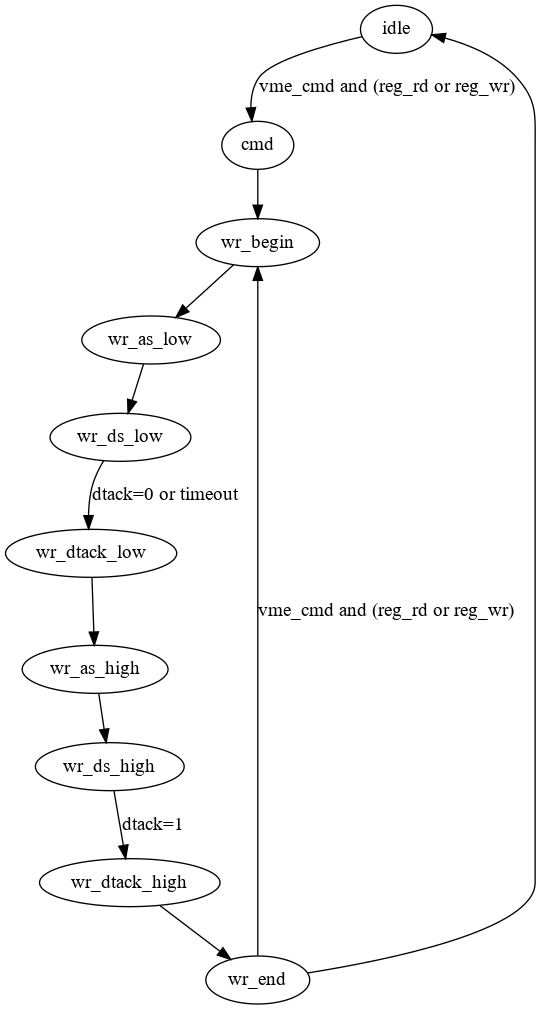
\includegraphics[width= 0.4 \textwidth]{figures/vmestates.png}
\caption{Simulated VME state machine}
\label{fig:vmestatemachine}
\end{figure}

\subsection{DCFEB Simulation}

\texttt{dcfeb\_v6.vhd} contains a simulation of both DCFEB JTAG and fake-data generation functionality. The \texttt{bgb\_scan\_emulator} module directly takes in the JTAG inputs TMS and TDI and decodes the input JTAG signals. User commands (``\texttt{0x3C2}'') are decoded by the module \texttt{instr\_decode}, which then outputs a signal called \texttt{FSEL}. This goes to the modules that execute the different user commands such as \texttt{usr\_wr\_reg}, which handles ADC mask write command \texttt{0x0c}, \texttt{user\_cap\_reg}, which handles the BPI status command \texttt{0x17}, and the new \texttt{user\_counter\_reg}, which handles read counter commands \texttt{0x3B} and \texttt{0x3C}.

\section{ODMB Software}
%\bibliography{writeup}
%\bibliographystyle{plain}
%cite CMS paper https://iopscience.iop.org/article/10.1088/1748-0221/3/08/S08004/meta

%clk, fifoclk <= 40 MHz clock
%data_to_fifo <= load_data_cntr - just counts from 0 to 0x40 (64)
%startaddr <= startaddr (0x003cf960)
%startaddrvalid <= startaddrvalid
%	if (load_bit_cntr < 10) startaddrvalid <= '1' else '0'
%	load_bit_cntr just starts at 0 and counts up... so first 10 clk40 cycles?
%pagecount <= pagecount ("00000000000000001")
%pagecountvalid <= pagecountvalid '1' for first 10 clk40 cycles, then 0
%sectorcount <= "00000000000001"
%sectorcountvalid <= '1' for first 10 clk40 cycles, then 0
%fifowren '1' when load_bit_cntr < 64, '0' for 1 cycle at 64
%fifofull (to ILA)
%fifoempty (unused)
%fifoafull (unused)
%fifowrerr <= overflow (unused)
%fifoorderr <= underflow (unused)
%writedone (to ILA)
%reset <= '0'
%read <= pulsed from vio
%erase <= pulsed from vio
%eraseing (to ILA)
%out_read_inprogress (to ILA)
%in_CmdIndex - from Vio
%in_rdAddr - from Vio
%in_wdlimit - from Vio
%...
%
%vio -> startinfo, startdata, starterase, startread
%	ila_CmdIndex, ila_rdAddr, ila_wdlimit, vio_reset

%
\begin{table}[H]
\centering
\begin{tabular}{|l|l|} \hline
Port& Description\\ \hline
\texttt{CLK}& 40MHz clock\\ \hline
\texttt{RST}& reset signal input from top level\\ \hline
\texttt{BPI\_BANK\_BLOCK}& block where registers are stored, 0x0FF7 for CFG and 0x0FD7 for CONST\\ \hline
\texttt{BPI\_CFG\_REG\_WE\_O}& signal to indicate write to CFG registers to\\
                             & \texttt{CC\_CFG\_REG\_WE} on VMECONFREGS\\ \hline
\texttt{BPI\_CFG\_REGS}& value of CFG registers from VMECONFREGS\\ \hline
\texttt{BPI\_CFG\_DL\_START}& signal to download CFG registers from BPI\_PORT\\ \hline
\texttt{BPI\_CFG\_UL\_START}& signal to upload CFG registers from BPI\_PORT\\ \hline
\texttt{BPI\_DONE}& done signal from BPI\_CTRL\\ \hline
\texttt{BPI\_STATUS}& status from BPI\_CTRL\\ \hline
\texttt{BPI\_DIS}& multiplexed with disable signal from BPI\_PORT and sent to BPI\_CTRL\\ \hline
\texttt{BPI\_EN}& multiplexed with enable signal from BPI\_PORT and sent to BPI\_CTRL\\ \hline
\texttt{BPI\_CFG\_REG\_WE\_I}& write enable input from BPI\_CTRL\\ \hline
\texttt{BPI\_CFG\_BUSY}& output indicating busy to BPI\_PORT and VMECONFREGS\\ \hline
\texttt{BPI\_CMD\_FIFO\_WE}& multiplexed with write enable from BPI\_PORT and sent to BPI\_CTRL\\ \hline
\texttt{BPI\_CMD\_FIFO\_IN}& multiplexed with fifo data from BPI\_PORT and sent to BPI\_CTRL\\ \hline
\end{tabular}
\caption{Signals on BPI\_CFG\_CONTROLLER module}
\label{tab:cfgcontrollerinterface}
\end{table}

\end{document}
